\addcontentsline{toc}{section}{Appendix} % Remove this if you don't want the appendix included in the table of contents.
\appendix

\section{MATLAB Code}\label{sec:matlab}
\subsection{plot\_constraint.m}\label{sec:plot_constraint_m}
\lstinputlisting{code/plot_constraint.m}

\subsection{problem2.m}\label{sec:problem2_m}
\lstinputlisting{problem2/problem2.m}

\subsection{problem3.m}\label{sec:problem3_m}
\lstinputlisting{problem3/ex3_1.m}
\lstinputlisting{problem3/ex3_2.m}


\subsection{problem4.m}\label{sec:problem4_m}
\lstinputlisting{problem4/ex4.m}
\lstinputlisting{problem4/nonlcon.m}
\lstinputlisting{problem4/ex4_4.m}
\lstinputlisting{problem4/ex4_4_CL.m}
\lstinputlisting{problem4/ex4_4_OL.m}



\section{Simulink Diagrams}\label{sec:simulink}
This section should contain your Simulink diagrams. Just like the plots, these should be in vector format, like in \Cref{fig:simulink}. Make them tidy enough to understand.


\begin{figure}[htb]
	\centering
		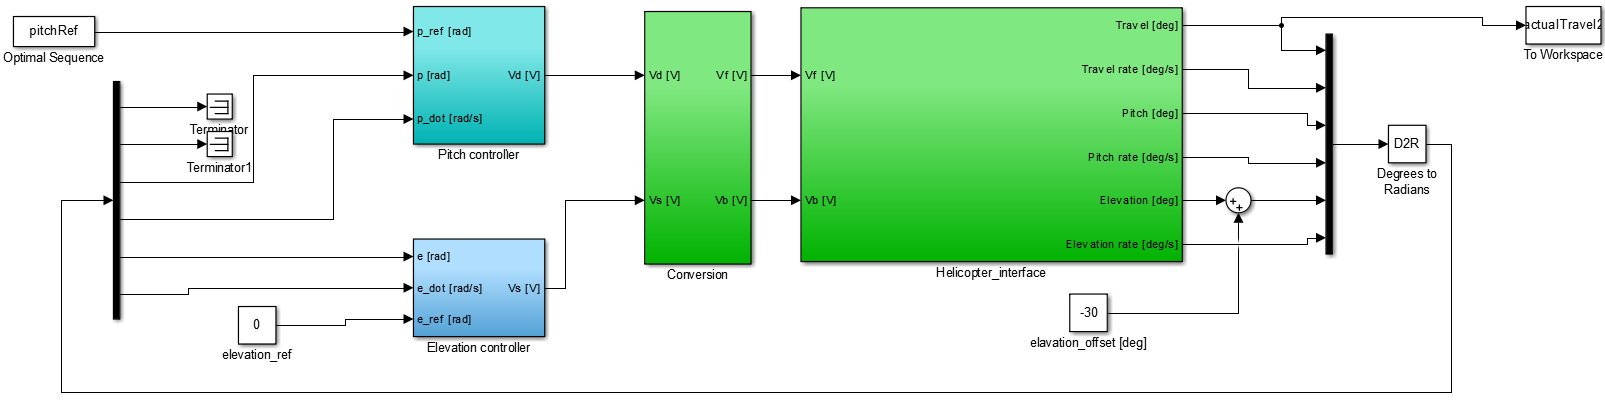
\includegraphics[width = \textwidth]{figures/simulink/oppgave2.PNG}
	\caption{Problem 2, pitch/travel open loop}
\label{fig:problem2}
\end{figure}

\begin{figure}[htb]
	\centering
		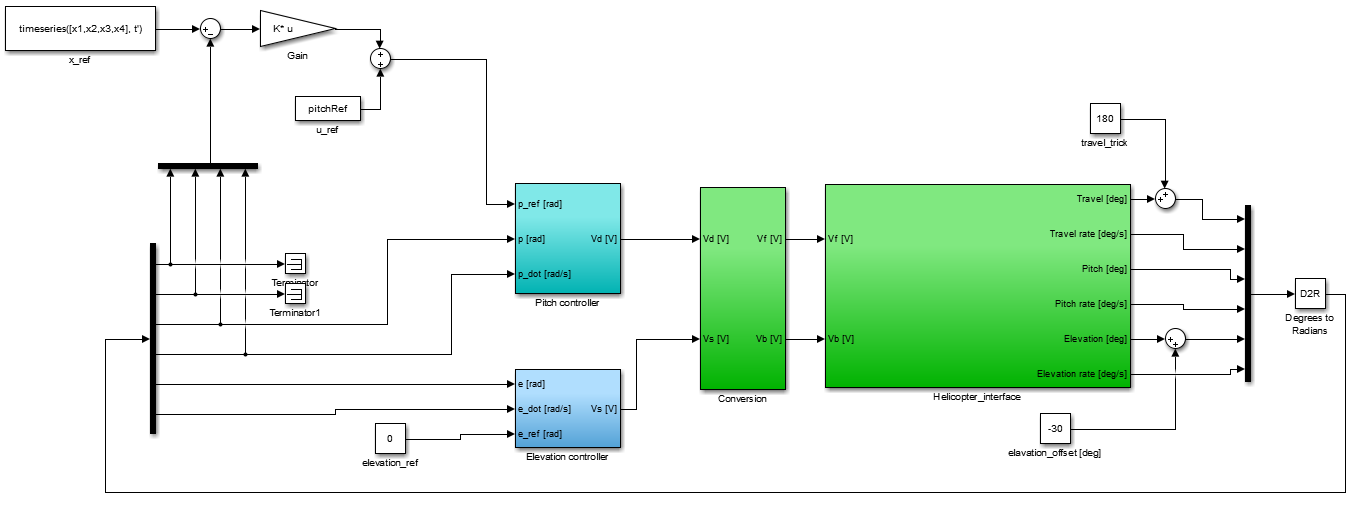
\includegraphics[width = \textwidth]{figures/simulink/problem3.PNG}
	\caption{Problem 3, pitch/travel closed loop}
\label{fig:problem3}
\end{figure}

\begin{figure}[htb]
	\centering
		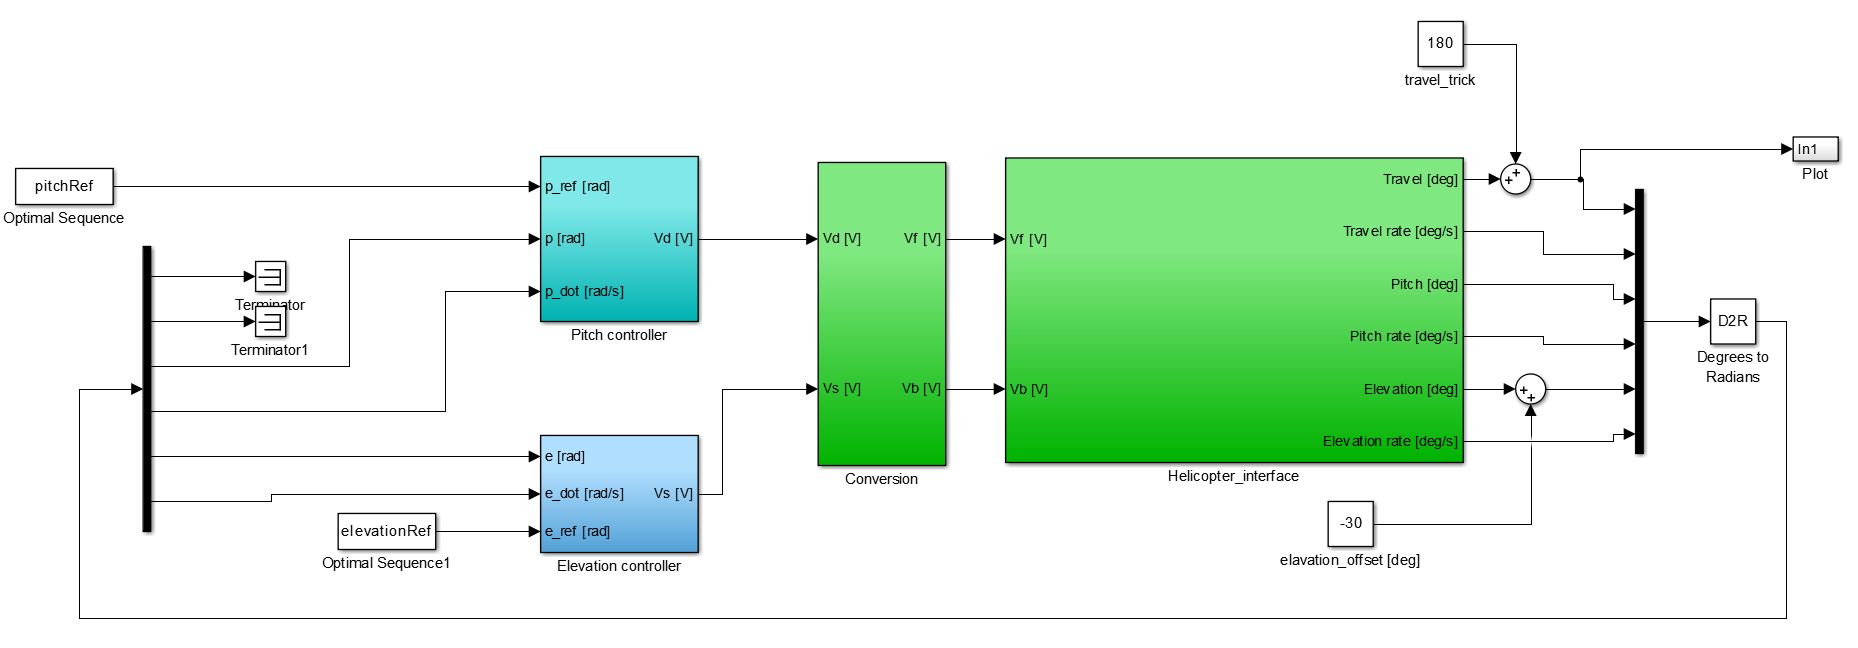
\includegraphics[width = \textwidth]{figures/simulink/problem4_OL.PNG}
	\caption{Problem 4, pitch/travel and elevation, Open loop}
\label{fig:problem4_OL}
\end{figure}

\begin{figure}[htb]
	\centering
		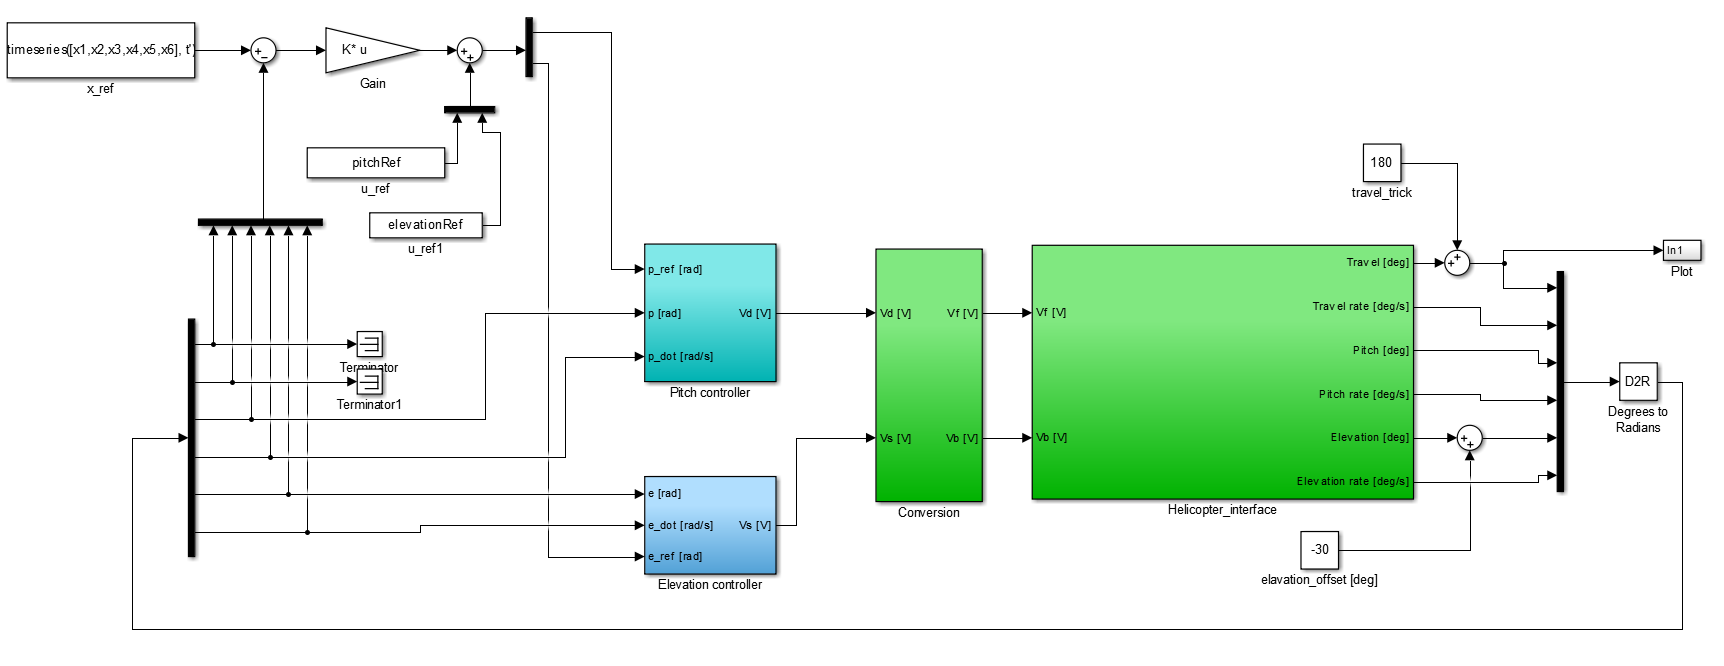
\includegraphics[width = \textwidth]{figures/simulink/problem4_CL.PNG}
	\caption{Problem 4, pitch/travel and elevation, closed loop}
\label{fig:problem4_CL}
\end{figure}
